\documentclass{article}
\usepackage[utf8]{inputenc}
\usepackage[T1]{fontenc}
\usepackage[utf8]{inputenc}
\usepackage{graphicx}
\usepackage[a4paper, total={6.5in, 8.6in}]{geometry}
\setcounter{secnumdepth}{4}
\usepackage{hyperref}
\usepackage{color}
\usepackage{booktabs}
\usepackage{tabularx}
\usepackage{amsmath}
\usepackage{textcomp}
\usepackage{xcolor}
\usepackage{listings}
\usepackage{enumitem}
\usepackage{minted}
\usepackage{tikz}
\usepackage{ccicons}
\usepackage{fancyhdr}
\usepackage{pgfplots}
\usepackage[
type={CC},
modifier={by-nc-sa},
version={4.0},
]{doclicense}
\pgfplotsset{compat=newest}
\usetikzlibrary{arrows.meta, positioning}

\definecolor{highlight}{rgb}{0.22,0.45,0.70}

\title{Classification of Room Occupancy using a Convolutional Neural Network}
\author{Alessandro Amella}
\date{\today}

\makeindex

\pagestyle{fancy}
\fancyhf{} % Clear header and footer
\fancyhead[C]{\nouppercase{\leftmark}} % Current section at the top
\fancyfoot[C]{\thepage} % Page numbers at the bottom 
\renewcommand{\headrulewidth}{0.4pt} % Header rule
\renewcommand{\footrulewidth}{0pt} % Footer rule

\begin{document}

\maketitle

\begin{abstract}
    This report presents the development process and performance evaluation of a convolutional neural network (CNN) model for classifying room occupancy based on 60 GHz signal transmissions. The model was trained on labeled delay-Doppler snapshots and optimized using hyperparameter tuning techniques. The report provides a detailed description of the problem, data preprocessing steps, model architecture, hyperparameter optimization using Optuna, and the achieved results. The final model demonstrates high accuracy in classifying the number of persons in a room based on the given delay-Doppler snapshots.
\end{abstract}

\begin{center}
    \includegraphics[height=1.5cm]{vut.png} % Adjust height as needed
    \hspace{1cm} % Adjust horizontal space between images
    \includegraphics[height=1.5cm]{fekt.png} % Adjust height as needed
\end{center}

\doclicenseThis%

\begin{center}
    \footnotesize{The VUT logo and all associated trademarks are the property of Vysoké učení technické v Brně. All rights reserved.}
\end{center}

\tableofcontents

\clearpage


\section{Introduction}
The ability to accurately classify the number of persons in a room has significant applications in various domains, such as energy management, security systems, and smart environments. Traditional methods for occupancy detection often rely on intrusive sensors or manual counting, which can be inefficient and raise privacy concerns. In recent years, the use of wireless signals, particularly in the 60 GHz frequency range, has emerged as a promising approach for non-intrusive occupancy detection.

This project aims to develop a machine learning model capable of classifying the number of persons in a room based on 60 GHz signal transmissions. By analyzing delay-Doppler snapshots that capture the reflections from targets (humans/machines) at varying distances and velocities, the model can distinguish between four occupancy classes: machine only (zero persons), one person, two persons, and three persons in the room.

The development of an accurate and reliable occupancy classification model has several potential benefits. It can enable energy-efficient control of heating, ventilation, and air conditioning (HVAC) systems by adjusting settings based on the actual occupancy level. In security applications, the model can help detect unauthorized presence or unusual occupancy patterns. Furthermore, it can contribute to the development of smart environments that adapt and respond to the presence and activities of occupants.

This report presents the methodology, implementation details, and results of developing a convolutional neural network (CNN) model for room occupancy classification. The report is structured as follows: Section 2 provides a detailed description of the problem and the dataset used. Section 3 explains the methodology, including data preprocessing, model architecture, and hyperparameter optimization. Section 4 presents the results, discussing the hyperparameter tuning process and the final model's performance. Section 5 concludes the report and suggests potential future improvements.

\section{Problem Description}
The dataset used in this project consists of delay-Doppler snapshots representing 60 GHz signal transmissions in a room. Each snapshot is a two-dimensional image in PNG format, capturing the reflections from targets (humans/machines) at different distances and velocities relative to the receiver.

In a delay-Doppler snapshot, the horizontal axis represents the delay, indicating the distance of the target from the receiver. The vertical axis represents the Doppler frequency shift, which is related to the velocity of the target. Targets that are farther away from the receiver generate higher delays, while targets moving faster generate higher Doppler frequency shifts.

Figure \ref{fig:snapshots} shows examples of delay-Doppler snapshots for different room occupancy scenarios. The snapshots on the left, middle, and right correspond to one person, two persons, and three persons in the room, respectively. These examples represent ideal cases where the targets are clearly distinguishable. However, in real-world scenarios, the snapshots may be distorted by noise, reflections from objects, and missed targets, making the classification task more challenging.

\begin{figure}[H]
    \centering
    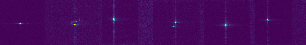
\includegraphics[width=0.8\textwidth]{training_data_example.png}
    \caption{Examples of delay-Doppler snapshots for different room occupancy scenarios.}
    \label{fig:snapshots}
\end{figure}

The objective of this project is to develop a machine learning model that can accurately classify the number of persons in a room based on these delay-Doppler snapshots. The model should be able to distinguish between four occupancy classes:

\begin{itemize}
    \item Machine only (zero persons in the room)
    \item One person in the room
    \item Two persons in the room
    \item Three persons in the room
\end{itemize}

The dataset is divided into training and testing sets. The training set consists of labeled delay-Doppler snapshots along with their corresponding occupancy classes. The testing set contains unlabeled snapshots for which the model needs to predict the occupancy class. The performance of the model will be evaluated based on its accuracy in classifying the snapshots in the testing set.

\section{Methodology}
The development of the room occupancy classification model involved several key steps, including data preprocessing, designing the CNN architecture, and optimizing hyperparameters using Optuna. This section provides a detailed description of each step.

\subsection{Data Preprocessing}
Data preprocessing is a crucial step in preparing the input data for training the CNN model. The delay-Doppler snapshots are provided as PNG images, and several preprocessing techniques were applied to ensure consistent and suitable input for the model.

Firstly, the training data was loaded from the PNG images using the Python Imaging Library (PIL). Each image was converted from its original format to RGB to ensure a consistent color space representation.

Next, the images were cropped to remove any white borders surrounding the actual delay-Doppler snapshot. The cropping was performed by removing 2 pixels from each side of the image, effectively eliminating the white border.

To ensure a consistent input size for the CNN model, the cropped images were resized to a fixed dimension of 50x44 pixels. This resizing step guarantees that all snapshots have the same spatial dimensions, facilitating batch processing during training and inference.

Finally, the pixel values of the resized images were normalized to a range between 0 and 1. Normalization helps to improve the convergence of the model during training by scaling the input values to a consistent range.

After preprocessing, the training data was split into two subsets: a training set and a validation set. The validation set was used to evaluate the model's performance during training and to prevent overfitting. The split ratio was set to 80\% for training and 20\% for validation.

\subsection{Model Architecture}
The choice of model architecture plays a significant role in the performance of the room occupancy classification task. Convolutional Neural Networks (CNNs) have proven to be highly effective in image classification tasks due to their ability to capture spatial hierarchies and learn discriminative features.

The CNN architecture used in this project consists of multiple layers, including convolutional layers, max pooling layers, flatten layers, and dense layers. Figure \ref{fig:architecture} illustrates the overall architecture of the model.

\begin{figure}
    \centering
    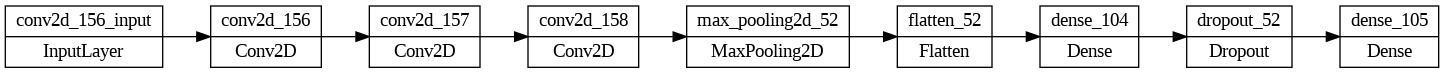
\includegraphics[width=1\textwidth]{model_plot.png}
    \caption{CNN architecture used for room occupancy classification.}
    \label{fig:architecture}
\end{figure}


The input to the model is a preprocessed delay-Doppler snapshot with dimensions of 50x44 pixels and three color channels (RGB). The first layer is a convolutional layer with a specified number of filters (determined during hyperparameter tuning) and a kernel size of 3x3. The convolutional layer applies learnable filters to the input image, capturing local spatial patterns and generating feature maps.

The output of the convolutional layer is passed through a Rectified Linear Unit (ReLU) activation function, which introduces non-linearity into the model and helps in learning complex patterns. The ReLU activation function sets negative values to zero, allowing the model to focus on positive activations.

The model includes multiple convolutional layers, each followed by ReLU activation, to learn hierarchical features at different scales. The number of filters in each convolutional layer is determined during hyperparameter tuning.

After the convolutional layers, a max pooling layer is applied to reduce the spatial dimensions of the feature maps. Max pooling selects the maximum value from a local neighborhood, helping to extract the most prominent features and provide translation invariance.

The output of the max pooling layer is flattened into a one-dimensional vector, which is then passed through dense layers. The dense layers learn high-level features and perform the final classification. The number of units in the dense layers is determined during hyperparameter tuning.

To prevent overfitting and improve generalization, dropout regularization is applied after the dense layers. Dropout randomly sets a fraction of the input units to zero during training, forcing the model to learn more robust features.

The final dense layer has four units, corresponding to the four occupancy classes. A softmax activation function is applied to the output of this layer, producing a probability distribution over the classes. The class with the highest probability is considered the predicted occupancy class.

The model is compiled with the Adam optimizer, which adaptively adjusts the learning rate during training. The loss function used is categorical cross-entropy, which is suitable for multi-class classification problems. The model's performance is evaluated based on accuracy, which measures the proportion of correctly classified snapshots.

\subsection{Hyperparameter Optimization}
Hyperparameter optimization is the process of finding the best combination of hyperparameters that maximizes the model's performance. In this project, Optuna, an automatic hyperparameter optimization framework, was used to search for the optimal hyperparameters.

Optuna allows defining an objective function that takes hyperparameters as input and returns a performance metric, such as validation accuracy. The objective function specifies the search space for each hyperparameter, and Optuna explores this space to find the best combination.

The hyperparameters considered for optimization in this project include:

\begin{itemize}
    \item Number of convolutional filters: The number of filters in each convolutional layer determines the depth of the feature maps and the model's capacity to learn patterns. A higher number of filters can capture more complex features but may also increase the risk of overfitting.
    \item Number of dense units: The number of units in the dense layers affects the model's ability to learn high-level features and make predictions. A larger number of units can model more complex relationships but may also lead to overfitting.
    \item Dropout rate: The dropout rate determines the fraction of input units that are randomly set to zero during training. Dropout helps in regularizing the model and preventing overfitting. A higher dropout rate can improve generalization but may slow down convergence.
    \item Learning rate: The learning rate controls the step size at which the model's weights are updated during training. A higher learning rate can lead to faster convergence but may cause the model to overshoot the optimal solution. A lower learning rate can result in slower convergence but may help in finding a better local minimum.
\end{itemize}

Optuna was configured to maximize the validation accuracy as the objective metric. The search space for each hyperparameter was defined based on prior knowledge and empirical observations. For example, the number of convolutional filters was set to a categorical choice of [32, 64, 128], while the learning rate was sampled from a log-uniform distribution between 1e-5 and 1e-2.

During the optimization process, Optuna generated trial configurations by sampling hyperparameter values from the defined search spaces. Each trial configuration was used to create a new instance of the CNN model, which was then trained on the training set and evaluated on the validation set. The validation accuracy achieved by each trial was recorded and used to guide the search for better hyperparameters.

Optuna employs various optimization algorithms, such as Tree-structured Parzen Estimator (TPE) and CMA-ES, to efficiently explore the hyperparameter space and find promising configurations. The optimization process was run for a specified number of trials or until a satisfactory level of performance was achieved.

After the optimization process, the best hyperparameters found by Optuna were used to train the final model on the entire training set. The performance of the final model was then evaluated on the held-out testing set to assess its generalization ability.

\section{Results}

\subsection{Hyperparameter Tuning}
The hyperparameter tuning process using Optuna resulted in the discovery of the best hyperparameters for the CNN model. The optimal values found for each hyperparameter are as follows:

\begin{itemize}
    \item Number of convolutional filters: 128
    \item Number of dense units: 512
    \item Dropout rate: 0.2367
    \item Learning rate: 0.0001191
\end{itemize}

These hyperparameters were determined based on the validation accuracy achieved during the optimization process. Optuna explored various combinations of hyperparameters and found the configuration that yielded the highest validation accuracy.

Figure \ref{fig:optimization} shows the progress of the hyperparameter optimization process. The figure illustrates the validation accuracy achieved by each trial configuration over the course of the optimization. The best trial, indicated by the red marker, corresponds to the hyperparameters mentioned above.

\begin{figure}
    \centering
    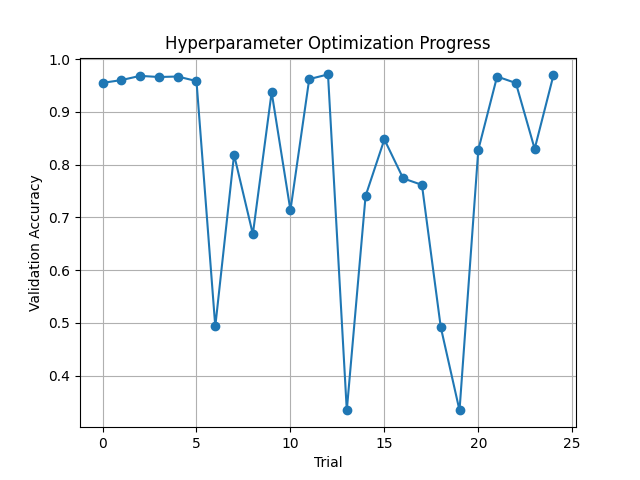
\includegraphics[width=0.7\textwidth]{hyperparameter_optimization.png}
    \caption{Hyperparameter optimization progress using Optuna.}
    \label{fig:optimization}
\end{figure}

\subsection{Model Performance}
Using the best hyperparameters found through optimization, the final CNN model was trained on the entire training set. The model's performance was evaluated on the held-out testing set to assess its generalization ability.

Figure \ref{fig:accuracy} presents the training and validation accuracy curves during the training process. The model achieved a high training accuracy, indicating its ability to learn patterns from the training data. The validation accuracy also improved over the epochs, suggesting that the model generalizes well to unseen data.

\begin{figure}
    \centering
    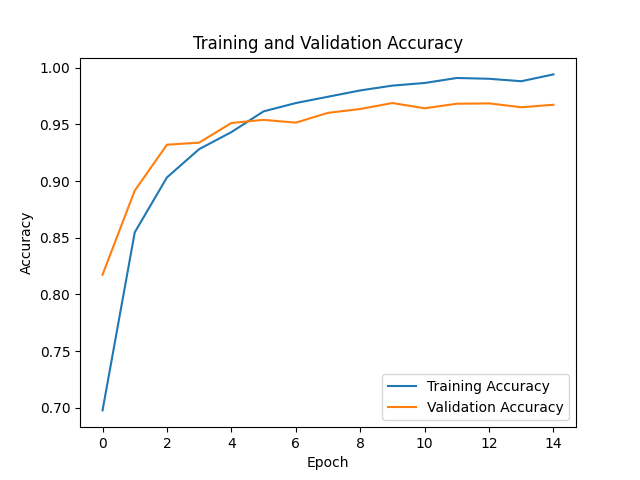
\includegraphics[width=0.7\textwidth]{accuracy_curves.png}
    \caption{Training and validation accuracy curves during model training.}
    \label{fig:accuracy}
\end{figure}

The final model achieved a testing accuracy of 96.94\% on the held-out testing set. This accuracy demonstrates the model's capability to accurately classify the number of persons in a room based on the delay-Doppler snapshots.

Figure \ref{fig:confusion_matrix} shows the confusion matrix for the model's predictions on the testing set. The confusion matrix provides insights into the model's performance for each occupancy class. The rows represent the true classes, while the columns represent the predicted classes. The values in the matrix indicate the number of snapshots classified into each category.

\begin{figure}
    \centering
    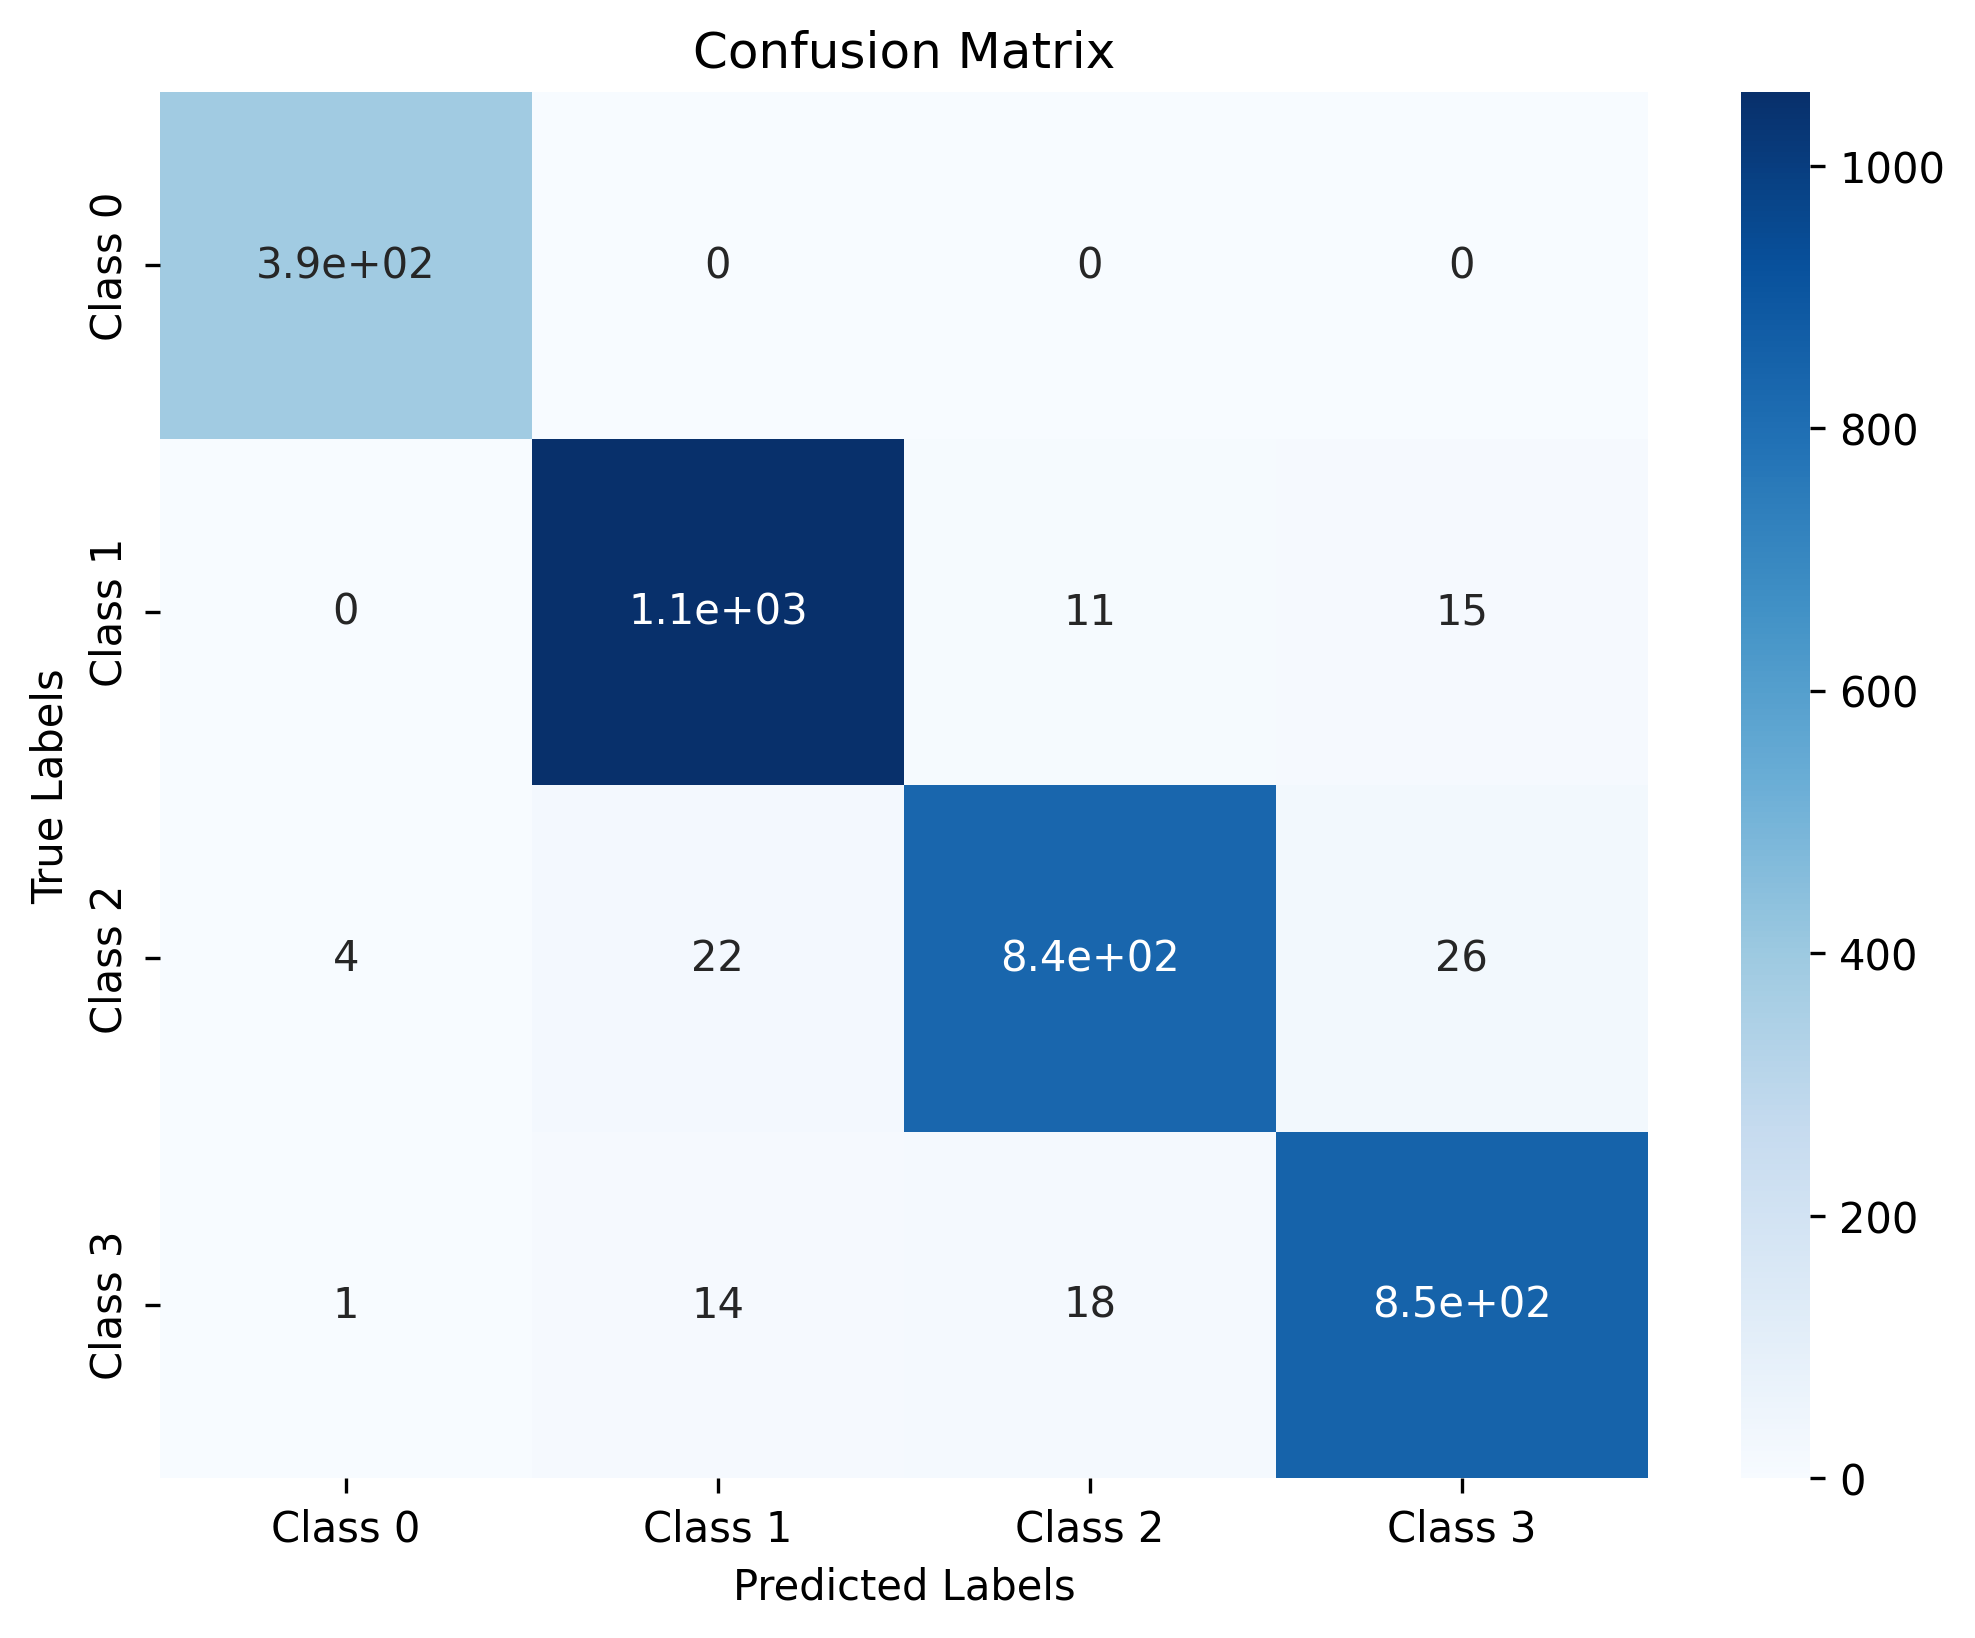
\includegraphics[width=0.7\textwidth]{confusion_matrix.png}
    \caption{Confusion matrix for the model's predictions on the testing set.}
    \label{fig:confusion_matrix}
\end{figure}

\section{Conclusion}
The CNN model, optimized using Optuna, achieved a high validation accuracy of 96.94\%. This work advances occupancy detection for applications in smart environments, security systems, and others. The source code is available on GitHub \textcolor{blue}{\href{https://github.com/Bitrey/MLBrno/blob/master/Project/Project.ipynb}{here}}.

\vspace*{\fill}

\vspace{2em}
\hrulefill
\vspace{1em}

\textbf{Alessandro Amella \textcopyright{} 2024}

\end{document}